\documentclass[twocolumn]{article}

\usepackage{graphicx} % Required for inserting images
\usepackage{multicol}
\usepackage{placeins}
\usepackage{amsfonts}
\usepackage{amsmath}
\usepackage{amsthm}
\usepackage{listings}
\usepackage{amssymb}
\usepackage[a4paper, left=0.5in, right=0.5in, top=0.6in, bottom=0.6in]{geometry}
\usepackage{xcolor}
\usepackage{tikz}
\usepackage{float}
\usepackage{caption}
\usepackage{booktabs}
\usepackage{hyperref}
\usepackage{url}
\usepackage{breakurl}
\usepackage{sectsty}
\usepackage[]{helvet}
\usepackage{titling}
\usepackage{enumitem}
\usepackage{titlesec}

\titlespacing*{\section}{0pt}{0.9ex}{0.9ex}
\titlespacing*{\subsection}{0pt}{0.7ex}{0.7ex}
\titlespacing*{\subsubsection}{0pt}{0.7ex}{0.7ex}

%\allsectionsfont{\sffamily\bfseries}
\pretitle{\begin{center}\sffamily\bfseries\Large}
\posttitle{\par\end{center}}
\preauthor{\begin{center}\sffamily\bfseries}
\postauthor{\par\end{center}}
\predate{\begin{center}\sffamily\bfseries}
\postdate{\par\end{center}}

\usetikzlibrary{automata, positioning, arrows.meta}

\renewcommand{\leq}{\leqslant}
\renewcommand{\geq}{\geqslant}
\renewcommand{\le}{\leqslant}
\renewcommand{\ge}{\geqslant}
\newcommand{\vsp}{\vspace{0.5em}}
\newcommand{\expect}{\mathbb{E}}
\newcommand{\prob}{\mathbf{P}}
\newcommand{\ruler}{
    \vspace{1em}
    \hrule
    \vspace{1em}
}
\newcommand{\bsq}{\hfill $\blacksquare$}


\lstset{
    language=C++,          % Set the language for syntax highlighting
    numbers=left,          % Display line numbers on the left
    numberstyle=\tiny\color{gray},  % Style for line numbers
    rulecolor=\color{black},         % Border color around the code block
    basicstyle=\ttfamily\footnotesize, % Set font style and size (smaller font)
    keywordstyle=\color{blue},   % Syntax highlighting for keywords
    commentstyle=\color{green},  % Syntax highlighting for comments
    stringstyle=\color{red},   % Syntax highlighting for strings
    morekeywords={auto, register, inline}, % Add extra C++ keywords if necessary
}

\title{Algorithm Selection: A Predictive Model for Optimal Sorting}
\author{Artem Kiselev}

\begin{document}

\maketitle

\section{Introduction}
Sorting is a fundamental task that appears across various applications in computer science, from database management to data analytics and real-time processing systems. Due to its critical importance, hundreds of sorting algorithms have been developed, each with unique performance characteristics optimized for particular scenarios. Some algorithms excel at sorting nearly-sorted data, others at handling large datasets, and others at optimizing memory usage. As a consequence, no single algorithm universally outperforms all others for all problem instances. This naturally leads to the following research question:

\begin{quote}
\emph{Can we design a model that dynamically and intelligently selects the optimal sorting algorithm based on the characteristics of a given dataset?}
\end{quote}

Successfully addressing this question and constructing an effective predictive model would represent a meaningful advancement. Such a model, capable of analyzing a dataset's characteristics and predicting the optimal sorting strategy based on that analysis, could deliver substantial performance improvements over current static approaches. In practical terms, this could significantly enhance efficiency in real-world scenarios, including large-scale database operations, data-intensive computations, and latency-sensitive applications, providing tangible benefits over existing sorting implementations.

\section{Background and Problem \\ Formalization}
\subsection{Algorithm Selection Problem}
This question is an instance of the algorithm selection problem, formulated by John Rice in 1976 \cite{ricealgorithmselection}. It is formally stated as follows: 

\vsp

\noindent\textbf{Given:}
\begin{itemize}[itemsep=0.05em, topsep=0pt, leftmargin=1em]
    \item A problem space $\mathcal{P}$, containing all possible problem instances.
    \item A feature space $\mathcal{F}$, where each $f(x)\in\mathcal{F}$ represents measurable characteristics of problem $x\in\mathcal{P}$.
    \item An algorithm space $\mathcal{A}$, containing all applicable algorithms $A_i$.
    \item A performance space $\mathbb{R}^n$, where $p(A_i,x)$ represents the performance of algorithm $A_i\in\mathcal{A}$ on problem $x\in\mathcal{P}$.
    \item The final algorithm performance metric $||p||$, obtained by normalizing the raw performance measures.
\end{itemize}

\noindent\textbf{Find:} A selection mapping 
\[
S:\mathcal{F}\rightarrow\mathcal{A}
\]
that maximizes performance according to some criteria.

\subsection{Measures of Presortedness}
Before we discuss how the defined model applies to our research question, we must talk about measures of presortedness, which are a measurement of the pre-existing order of a list. A good measure of presortedness must satisfy the following criteria:

\vsp

\noindent \emph{Let $m$ be a measure of presortedness, and $X, Y$ be lists:}
\begin{enumerate}[itemsep=0.05em, topsep=0pt]
    \item $m(X) = 0$ if $X$ is \emph{fully sorted in ascending order}.
    \item If $X = [x_1, \cdots, x_n]$, $Y= [y_1, \cdots, y_n]$, and 
    \[
    x_i < x_j \iff y_i < y_j \quad \text{for all } i \text{ and } j,
    \]
    then $m(X) = m(Y)$.
    \item If $X \subseteq Y$, then $m(X) \leq m(Y)$.
    \item If $X < Y$, then $m(XY) \leq m(X) + m(Y)$.
    \item \emph{For any element} $a$, $m(a + X) \leq |X| + m(X)$.
\end{enumerate}

For this project, I will explicitly mention the following three measures of presortedness:

\vsp


\noindent \textbf{Runs \cite{Knuth1973}:}
The number of maximal contiguous ascending subsequences in a list $X$. 
\[
\text{Runs}(X) = \left|\{i : 1 \leq i < n \text{ and } a_{i+1} < a_i\}\right|.
\]
This takes $O(n)$ time, and $O(1)$ memory.

\ruler

\vsp

\noindent \textbf{Dis \cite{adaptivesortingsurvey}:}
The largest distance for which an inversion exists
\[
\text{Dis}(X) = \operatorname{max}\{j - i : 1 \leq i < j \leq n, x_i > x_j\}.
\]
This takes $O(n)$ time, and $O(n)$ memory.

\ruler

\vsp

\noindent \textbf{Mono \cite{zhang2016sortrace}:} 
The minimum number $k$ such that $X$ can be broken into $k$ subarrays where each subarray is \emph{monotonic}. A sequence is monotonic if it is increasing \emph{or} decreasing.
\[
\operatorname{Mono}(X)
=
\min\Bigl\{
k \in \mathbb{N}
:\,\exists\,1 = i_{0} < i_{1} < \cdots < i_{k} = n+1 :
\Bigr.
\]
\[
\Bigl.
\forall\, j \in \{1,\dots,k\},
(X_{i_{j-1}},\,X_{i_{j-1}+1},\dots,X_{i_{j}-1})
\text{ is monotonic}
\Bigr\}
\]

This takes $O(n)$ time, and $O(1)$ memory.
\ruler

\vsp

\noindent \textit{Note: }These are the only measures of presortedness that have a linear running time. This quality enables them to be used as features of lists for the problem of sorting.

\subsection{Other List Features}
Aside from the mentioned measures of presortedness, we define five other features:

\begin{enumerate}[itemsep=0.05em, topsep=0pt]
    \item \textbf{Size:} The total number of elements in the list, 
    \[
    \text{Size}(L) = |L|.
    \]
    
    \item \textbf{Average duplicates per unique element:} For a list $L$ with unique elements 
    $U$, if $|L| = n$, then
    \[
    \text{Avg. duplicates} = \frac{n - |U|}{|U|}.
    \]
    
    \item \textbf{Shannon entropy:} With frequency function $f(u)$ for $u\in U$ and $p(u)=\frac{f(u)}{n}$,
    \[
    H(L) = -\sum_{u\in U} p(u)\,\log_2 p(u).
    \]
    
    \item \textbf{Categorical skewness:} For categorical data—where each unique category $u\in U$ occurs with frequency $f(u)$ and the mean $\mu$ and standard deviation $\sigma$ are computed over these frequencies—the skewness is defined as 
    \[
    \gamma_1 = \frac{1}{|U|}\sum_{u\in U}\left(\frac{f(u)-\mu}{\sigma}\right)^3.
    \]
    This measure reflects the asymmetry of the frequency distribution for categorical variables.

    \item \textbf{Categorical kurtosis:} For categorical data with frequencies $f(u)$ for each $u\in U$, the kurtosis is defined by
    \[
    \gamma_2 = \frac{1}{|U|}\sum_{u\in U}\left(\frac{f(u)-\mu}{\sigma}\right)^4.
    \]
    This measure quantifies the tailedness of the frequency distribution for categorical variables.

\end{enumerate}

\subsection{Sorting Algorithm Selection Problem}
In our context, the problem space $\mathcal{P}$ consists of datasets that require sorting, and an instance $x \in \mathcal{P}$ is a list to be sorted. The feature space $\mathcal{F}$ is comprised of the size, categorical skewness, categorical kurtosis, Shannon entropy and, most importantly, the three measures of presortedness Runs, Dis, and Mono.

\vsp

Our algorithm space $\mathcal{A}$ includes various sorting algorithms like QuickSort, MergeSort, InsertionSort, and others. For simplicity, our performance space is defined as $\{0,1\}$, where a value of 1 indicates that the selection algorithm has correctly identified the fastest sorter for a given problem instance. We can now more formally state our research question:

\vsp

\noindent \textbf{Given:}
\begin{itemize}[itemsep=0.05em, topsep=0pt]
    \item Datasets $\mathcal{P} \ni x$, where $x$ is a list that requires sorting.
    \item A feature space $\mathcal{F}$, containing of the above stated features.
    \item An algorithm space $\mathcal{A}$, containing all applicable sorting algorithms $A_i$.
    \item A performance space $\{0,1\}$, where the performance metric is defined as
    \[
    p(A_i, x) = 
    \begin{cases}
    1, & \text{if } A_i \text{ is the fastest sorter for } x, \\
    0, & \text{otherwise.}
    \end{cases}
    \]
\end{itemize}

\noindent \textbf{Find:} A selection mapping
\[
S: \mathcal{F} \rightarrow \mathcal{A}
\]
that maximizes the average number of fastest sorter selections, i.e.,
\[
\max_{S} \frac{1}{|\mathcal{P}|} \sum_{x \in \mathcal{P}} p(S(f(x)), x).
\]

\section{Analysis and Implementation}
In this section, I reference specific files used to conduct the analysis, all of which can be found in the project's GitHub repository at 

\begin{center}
\href{https://github.com/kiselevart/sorting-selector/}{\texttt{github.com/kiselevart/sorting-selector/}}.
\end{center}

\subsection{cpp-sort Library Integration}
This project relies extensively on the \texttt{cpp-sort}\cite{cppsort_benchmarks} library, a C++ library featuring optimized implementations of various state-of-the-art sorting algorithms. Additionally, \texttt{cpp-sort} provides implementations of most measures of presortedness, referred to as probes.

To effectively leverage \texttt{cpp-sort} within Python, I created two separate interface files using \texttt{pybind11}: one file for interfacing with sorting algorithms and another dedicated to probes. These can be found in the \href{https://github.com/kiselevart/sorting-selector/tree/main/Implementation/src}{\texttt{src/}} directory. Utilizing \texttt{pybind11} allowed seamless integration of high-performance compiled C++ code into Python, thus maintaining Python's advantages in flexibility, extensive support for data science tasks, and ease of use within Jupyter Notebooks.

Before proceeding with the main analysis, I conducted preliminary benchmarks to ensure the reliability and efficiency of \texttt{cpp-sort}'s algorithms. The results from these benchmarks, detailed in \href{https://github.com/kiselevart/sorting-selector/blob/main/Implementation/analysis/verify_running_time.ipynb}{\texttt{verify\_running\_time.ipynb}}, confirmed that the chosen sorting methods performed consistently and significantly outperformed standard alternatives. Specifically, integrating the compiled sorters from \texttt{cpp-sort} provided, on average, a tenfold speedup compared to NumPy's sorting methods and over a fortyfold improvement compared to Python's built-in sorter.

\subsection{Sorters Redundancy Analysis}

After verifying the usability of the sorters within the \texttt{cpp-sort} library, I performed a "redundancy analysis" to identify and remove sorters that do not provide unique advantages over others. This process involved benchmarking various sorters across multiple datasets and visually analyzing performance graphs to detect any that were consistently outperformed. To confirm these observations, I conducted direct comparisons between selected algorithm pairs. The detailed analysis and graphs can be found in \href{https://github.com/kiselevart/sorting-selector/blob/main/Implementation/analysis/compare_sorts.ipynb}{\texttt{compare\_sorts.ipynb}}.

Based on this analysis, the following eight sorters were retained:
\begin{multicols}{2}
\begin{itemize}[itemsep=0.05em, topsep=0pt]
    \item \textbf{heap\_sort}
    \item \textbf{insertion\_sort}
    \item \textbf{merge\_sort}
    \item \textbf{quick\_sort}
    \item \textbf{quick\_merge\_sort}
    \item \textbf{spin\_sort}
    \item \textbf{std\_sort}
    \item \textbf{tim\_sort}
\end{itemize}
\end{multicols}

These selected sorters offer a diverse set of strategies and performance characteristics, ensuring robust and efficient sorting capabilities across various types of datasets.

\subsection{Probe Analysis}
The next step of the project involved an analysis of the available probes within the \texttt{cpp-sort} library. To achieve this, we computed the relative performance of each probe by evaluating the ratio between the execution time of each probe and the actual sorting time for every given list.

Formally, let $m_i$ represent a probe, $A_j$ a sorting algorithm, and $X_k \in X$ a specific list. Then, the ratio for a single list is defined as:
\[
    r_k = \frac{m_i(X_k)}{A_j(X_k)}
\]
The average ratio across all lists is computed as:
\[
    \bar{r} = \frac{1}{|X|}\sum_{k=1}^{|X|} r_k.
\]

The resulting heatmap visualization of these ratios can be accessed in \href{https://github.com/kiselevart/sorting-selector/blob/main/Implementation/analysis/probes_vs_sorts.ipynb}{\texttt{probes\_vs\_sorts.ipynb}}. Analysis of this heatmap, combined with considerations regarding the time complexity of all the presortedness measures clearly indicates that \texttt{Dis}, \texttt{Mono}, and \texttt{Runs} exhibit significantly superior efficiency. Thus, these three probes were selected for the feature space of the predictive model.

\section{Machine Learning and Results}
\label{sec:machine_learning}

After experimentally verifying the feature space, 
we synthesized a training dataset by computing all features in $\mathcal{F}$ and recording the 
fastest sorter for each list instance. Using these labeled data, we trained a classification 
model where the target variable was the fastest sorter. After exploring various algorithms and optimizing parameters, a Random 
Forest Classifier~\cite{breiman2001random} yielded the highest overall accuracy of $80.7\%$. 
Details on the training process can be found in 
\href{https://github.com/kiselevart/sorting-selector/blob/main/Implementation/analysis/train_model.ipynb}{\texttt{train\_model.ipynb}}.

\begin{figure}[htbp]
  \centering
  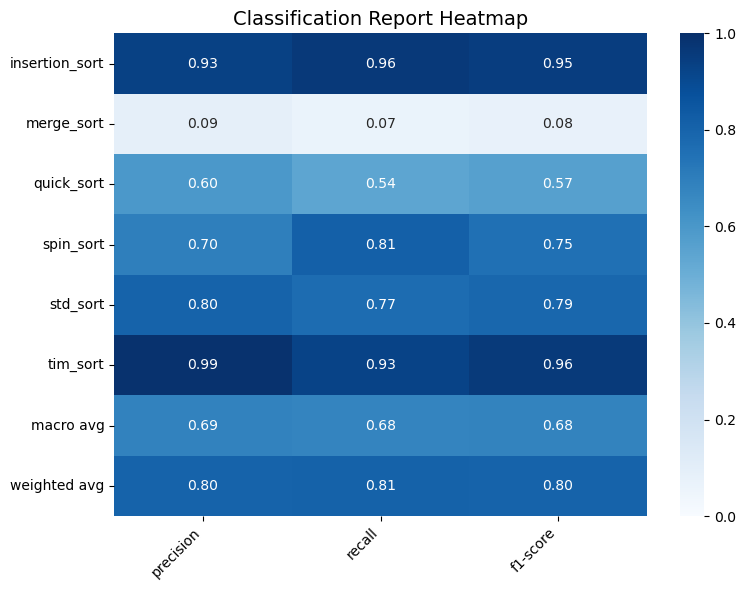
\includegraphics[width=0.48\textwidth]{../Implementation/figures/classification_report_heatmap.png}
  \caption{Classification Report Heatmap of the Random Forest Model}
  \label{fig:my_image}
\end{figure}

Figure~\ref{fig:my_image} shows a classification report heatmap for the trained model. The model 
classifies \texttt{tim\_sort} and \texttt{insertion\_sort} with notably high accuracy, likely 
because their performance characteristics differ distinctly from the other algorithms. By contrast, 
\texttt{merge\_sort} shows a high misclassification rate. 

One probable cause is a consistent performance spike around lists of size $750{,}000$ to $800{,}000$ 
elements, as shown in Figure~\ref{fig:merge_spike}. This spike may arise from caching or 
memory-access patterns specific to \texttt{merge\_sort}, which significantly degrades its performance 
in that narrow range of input sizes. Consequently, the model undervalues \texttt{merge\_sort} and 
fails to predict it even when it would otherwise be optimal.

\begin{figure}[htbp]
  \centering
  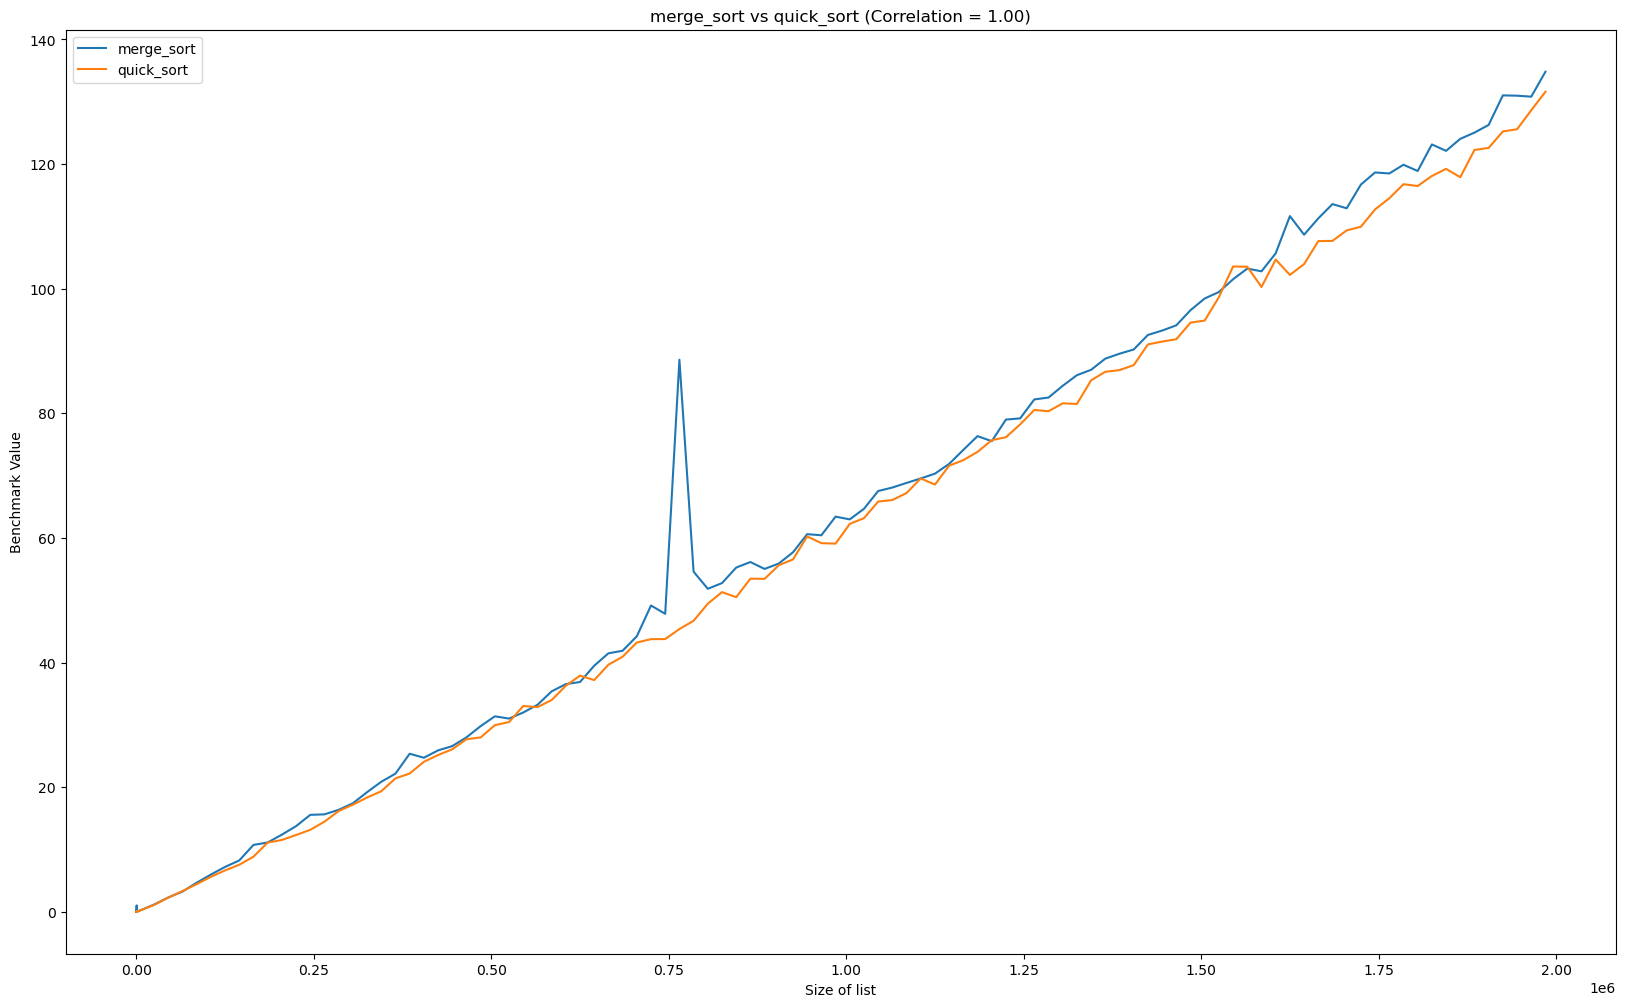
\includegraphics[width=0.48\textwidth]{../Implementation/figures/merge_sort_problem.png}
  \caption{Performance Spike of \texttt{merge\_sort} (blue) Around 750--800k Elements}
  \label{fig:merge_spike}
\end{figure}

Turning to feature importance (Figure~\ref{fig:features}), the three presortedness metrics 
clearly dominate as the most significant features. This aligns well with the intuition 
that knowing how close a list is to being sorted is critical when predicting the optimal 
sorting algorithm.

\begin{figure}[htbp]
  \centering
  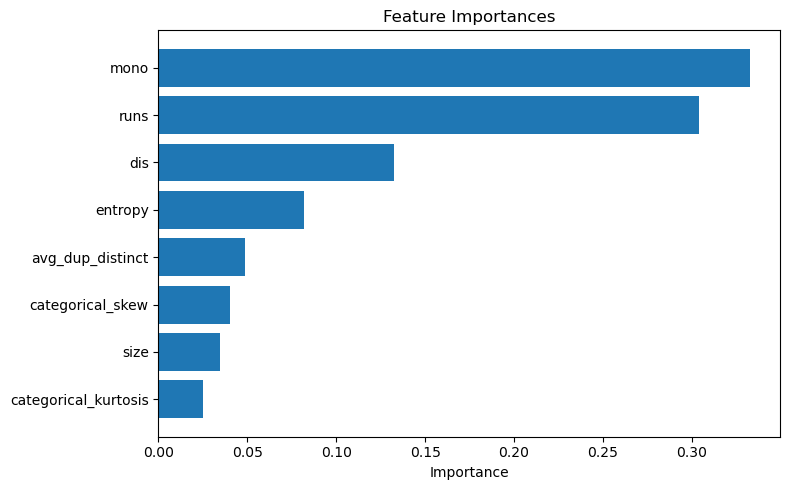
\includegraphics[width=0.45\textwidth]{../Implementation/figures/feature_importances.png}
  \caption{Feature Importances from the Random Forest Classifier}
  \label{fig:features}
\end{figure}

To further assess the model's performance in practice, Figure~\ref{fig:cases} compares the 
running time of the model's predicted sorter (blue) against each static sorter (orange) 
across $35{,}000$ test cases. While there are certain anomalies, the predictor generally 
runs comparably to the slower among the static sorters, which is a promising start for this initial 
model. Through implementing and researching the refinements that will be discussed below, there is a good chance that the predictive model could 
approach the performance of the optimal sorter on each instance.

\begin{figure}[htbp]
  \centering
  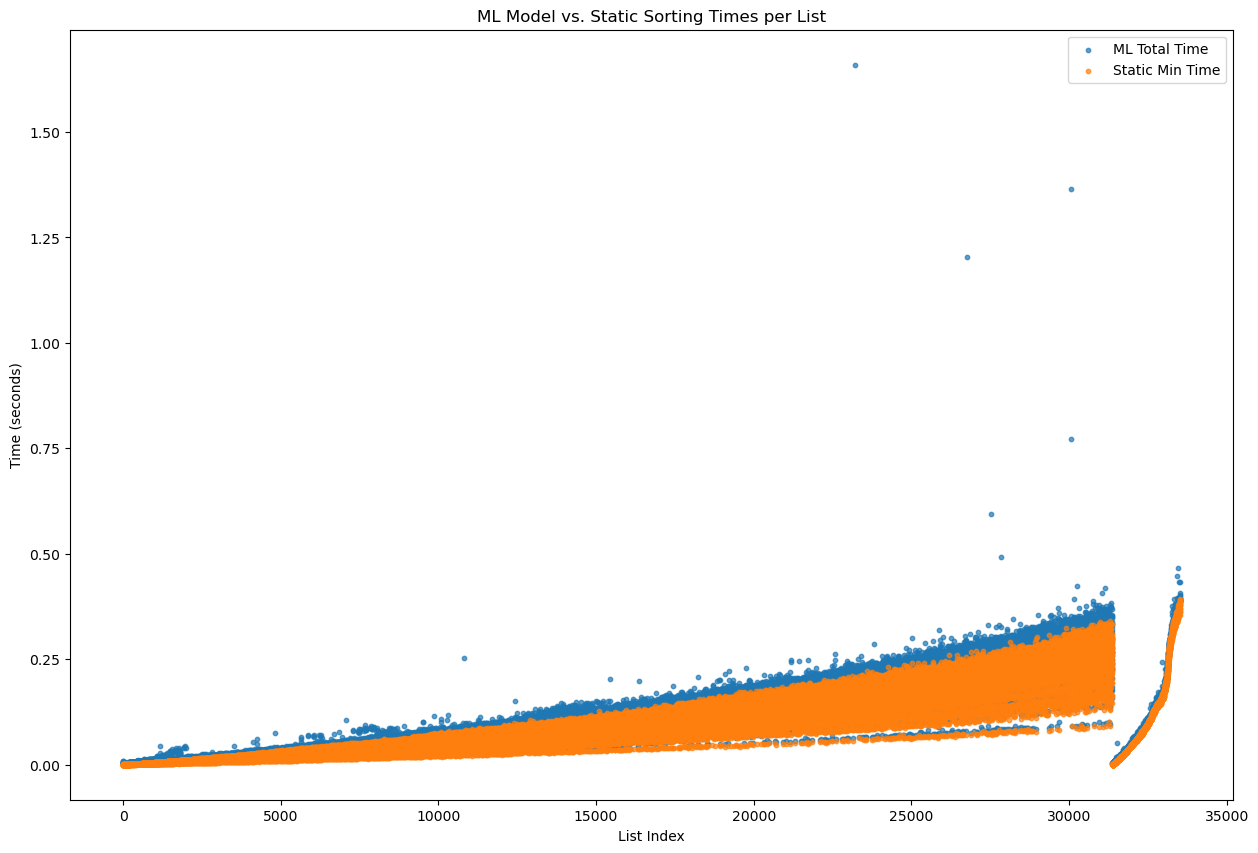
\includegraphics[width=0.45\textwidth]{../Implementation/figures/35000cases.png}
  \caption{Comparison of Model Predictions (blue) vs.\ Static Sorters (orange) Over 35,000 Cases}
  \label{fig:cases}
\end{figure}

\section{Further Work}
Due to the time constraints of this project, several improvements can be explored, along with numerous promising avenues for deeper research.

\subsection{Potential Improvements}
Several aspects of the current work could significantly benefit from enhancements, primarily in data quality and analytical methods. The datasets utilized throughout this project were synthetic, limiting the robustness of the results. Employing real-world data could substantially enhance the rigor and validity of the analysis. Furthermore, the synthetic datasets suffered from imbalances and were insufficiently large for training robust machine learning models. Increasing the dataset size and ensuring balanced class distributions could lead to more accurate and generalizable models.

Furthermore, the redundancy analysis of sorting algorithms relied predominantly on visual and graph-based inspections. While useful for exploratory analysis, such approaches may introduce biases and inaccuracies. Automating this step through statistical or algorithmic measures could reduce subjectivity and improve the reliability of the analysis. Lastly, the algorithm portfolio was significantly reduced for simplicity, which may have led to excluding potentially high-performing or contextually relevant algorithms. Expanding and rigorously evaluating a broader portfolio of sorting algorithms could yield more comprehensive and accurate insights.

\subsection{Areas for Deeper Research}
Several promising research directions could further extend the scope and applicability of this project:

\begin{itemize}
    \item \textbf{Enhanced Cost Functions:} Experimenting with more sophisticated or cost functions could lead to better model performance. For example, cost functions could aim to minimize the squared difference or absolute deviation between predicted sorter performance and the optimal sorter, rather than relying solely on categorical accuracy. 

    \item \textbf{Hybrid Model Development:} Investigating hybrid approaches that combine learned predictive models with manually engineered heuristics would almost certainly yield benefits. For instance, manually overriding the model's predictions with counting sort when inputs are known integers within a small, bounded range could enhance overall efficiency and accuracy.

    \vsp 
    \vsp

    \item \textbf{Approximation of Presortedness Metrics:} Developing methods to approximate presortedness could significantly enrich the feature space and thus improve model performance.

\end{itemize}

Each of these areas represents significant potential for deeper exploration and could substantially advance this research topic.

\section{Conclusion}
This project has successfully demonstrated the viability of using machine learning techniques to predict sorting algorithm performance based on input data features. Despite limitations due to synthetic data and algorithm simplifications, the results provided valuable insights and established a foundation for further enhancements. By addressing these limitations through improved data quality, expanded algorithm portfolios, and more rigorous analytical approaches, future research can significantly enhance predictive accuracy and robustness. 

Exploring advanced cost functions, hybrid models, presortedness metrics, and enhanced feature engineering promises to expand the utility and effectiveness of the predictive models developed. Successfully implementing these improvements could significantly enhance efficiency in real-world scenarios, including large-scale database operations, data-intensive computations, and latency-sensitive applications, providing tangible benefits over existing sorting implementations.

\bibliographystyle{plain}
\bibliography{references}

\end{document} 